\chapter{Аналитическая часть}

В данной части будет проводится анализ поставленной задачи, объектов трёхмерной сцены, а также существующие методы построения реалистических сцен.

\section{Задача n тел}
\subsection{Постановка задачи}
Пусть существует N частиц, представляемых материальными точками с массами $m_1, ..., m_N$, радиус векторами $\vec{r_1}, ..., \vec{r_N}$ и векторами скоростей $\vec{v_1}, ..., \vec{v_N}$ в момент времени $t=0$.
Попарное взаимойдействие точек подчинено закону тяготения ньютона:
\begin{equation}
	\label{eq:F_jk}
	\vec{F}_{jk} = G\hat{\vec{r_{jk}}}\frac{m_km_j}{\vec{r_{jk}}^2},
\end{equation}
где
\begin{itemize}
	\item $\vec{F}_{jk}$ - Сила тяготения, действующая j-ой частицой на k-ю;
	\item $G = 6.67430 * 10^{-11} m^3s^{-2}kg^{-1}$ - гравитационная постоянная, константа;
	\item $\vec{r_{jk}} = \vec{r_j} - \vec{r_k}$ - вектор из точки k-ой частицы в точку j-ой;
	\item $\hat{\vec{r_{jk}}}$ - единичный вектор из точки k-ой частицы в точку j-ой, задающий направление силы;
	\item $m_k, m_j$ - массы k-ой и j-oй частиц соответсвенно;
\end{itemize}

Так как на k-ю частицу действую все остальные частицы системы с силами (\ref{eq:F_jk}), а также с учётом того факта, что силы аддитивны, можно получить силу, с которой все частицы действую на k-ю:

\begin{equation}
	\label{eq:F_sumk}
	\vec{F}_{k} = Gm_k\sum_{j=1, j \neq k}^{N}{\frac{m_j}{\vec{r_{jk}}^2}\hat{\vec{r_{jk}}}}
\end{equation}

По второму закону Ньютона можно связать силу действующую на частицу с её ускорением:
\begin{equation}
	\label{eq:newton2}
	m\frac{d^2\vec{r}}{dt^2} = \vec{F},
\end{equation}
где
\begin{itemize}
	\item $m$ - масса частицы;
	\item $\vec{r}$ - радиус-вектор частицы;
	\item $\vec{F}$ - полная сила, действующая на частицу;
	\item $t$ - интервал времени.
\end{itemize}

Тогда объединив уравнения (\ref{eq:F_sumk}) и (\ref{eq:newton2}) получим уравнение движения k-ой частицы:
 
 \begin{equation}
 	\label{eq:r_k_before}
 	m_k\frac{d^2\vec{r_k}}{dt^2} = Gm_k\sum_{j=1, j \neq k}^{N}{\frac{m_j}{\vec{r_{jk}}^2}\hat{\vec{r_{jk}}}}
 \end{equation}
 или
 \begin{equation}
 	\label{eq:r_k_after}
 	\frac{d^2\vec{r_k}}{dt^2} = G\sum_{j=1, j \neq k}^{N}{\frac{m_j}{\vec{r_{jk}}^2}\hat{\vec{r_{jk}}}}
 \end{equation}
 
 Дифферинциальные уравнения второго порядка вида (\ref{eq:r_k_after}) всех частиц объединяются в систему уравнений:
  \begin{equation}
 	\label{eq:n_system}
 	\begin{cases}
 		\frac{d^2\vec{r_1}}{dt^2} = G\sum_{j=1, j \neq 1}^{N}{\frac{m_j}{\vec{r_{j1}}^2}\hat{\vec{r_{j1}}}} \\
 		\dots \\
 		\frac{d^2\vec{r_N}}{dt^2} = G\sum_{j=1, j \neq N}^{N}{\frac{m_j}{\vec{r_{jN}}^2}\hat{\vec{r_{jN}}}} \\
 	\end{cases}
 \end{equation}

Задачей N тел является решение системы уравнений (\ref{eq:n_system}) движения частиц с течением времени.
\subsection{Аналитические решения}
Для случаев $N = 1$ и $N = 2$ существуют точные аналитические решения, при этом для $N = 1$ по законам инерции частица будет двигаться прямолинено с постянной скоростью, а в случае $N = 2$ тела будут двигать по одной из кривых второго порядка: эллипсу, гиперболе или параболе.

Для случая $N = 3$ Г.Э. Брунс и А. Пуанкаре показали, что решение общее решение задачи невозможно выразить через алгебраические или через однозначные трансцендентные функции координат и скоростей тел \cite{markeev}. Однако в 1912 году Зульдман нашел точное решение задачи, но выраженный в виде бесконечных рядов, использовать которые, однако, невозвможно в следствие слишком высокой скорости роста кол-ва вычислений \cite{markeev}.

Для случаев $N \geq 3$ на текущий момент времени не было найдено точного аналитического решения ни в какой форме, однако существуют решения для определённых конфигураций
\subsection{Метод Эйлера}
Поскольку основная задача данной работы визуализация задачи n тел, а не поиск точного или максимального решения задачи n тел, то для решения системы уравнений (\ref{eq:n_system}) можно использовать самые простые численные методы. Одним из таких является метод эйлера, который и будет использоваться в данной работе.

Метод эйлера: для решения задачи Коши вида:
\begin{equation}
	\label{eq:koshi}
	\frac{dy}{dt} = f(t, y(t)), 0 \leq t \leq T, y(0) = y_0
\end{equation}
Введём на отрезке интегрирования сетку $\omega_\tau = {t_n = n\tau, n = 1,2,....}$, при этом будем обозначать $y_n = y(t_n)$  - сеточную функцию.
Тогда разностная схема эйлера:
\begin{equation}
	\label{eq:euler_frac}
	\frac{y_{n+1} - y_n}{\tau} = f(t_n, y_n)
\end{equation}
Все значения $y_i$, кроме $y_0$ ищутся итерационно по формуле:
\begin{equation}
	\label{eq:euler_formula}
	y_{n+1} = y_n + \tau f(t_n, y_n)
\end{equation}

Для применения метода эйлера для решения системы уравнений (\ref{eq:n_system}) приведём к системе дифференциальных уравнений первого порядка с помощью введения новых переменных - скоростей $v_i$ 

\begin{equation}
	\label{n_system_velocities}
	\begin{cases}
		\frac{d\vec{r_1}}{dt} = \vec{v_1} \\
		\dots \\
		\frac{d\vec{r_N}}{dt} = \vec{v_1} \\
		
		\frac{d\vec{v_1}}{dt} = G\sum_{j=1, j \neq 1}^{N}{\frac{m_j}{\vec{r_{j1}}^2}\hat{\vec{r_{j1}}}} \\
		\dots \\
		\frac{d\vec{v_N}}{dt} = G\sum_{j=1, j \neq N}^{N}{\frac{m_j}{\vec{r_{jN}}^2}\hat{\vec{r_{jN}}}} \\
	\end{cases}
\end{equation}

Такую систему можно решить методом эйлера используя формулу:
\begin{equation}
	\label{n_euler_velocities}
	\begin{cases}
		\vec{r}_{1(n+1)} = \vec{r}_{1(n)} + \tau \vec{v}_{1(n)} \\
		\dots \\
		\vec{r}_{N(n+1)} = \vec{r}_{N(n)} + \tau \vec{v}_{N(n)} \\
		
		
		\vec{v}_{1(n+1)} = \vec{v}_{1(n)} + \tau G\sum_{j=1, j \neq 1}^{N}{\frac{m_j}{\vec{r}_{j1(n)}^2}\hat{\vec{r}}_{j1(n)}} \\
		\dots \\
		\vec{v}_{N(n+1)} = \vec{v}_{N(n)} + \tau G\sum_{j=1, j \neq N}^{N}{\frac{m_j}{\vec{r}_{jN(n)}^2}\hat{\vec{r}}_{jN(n)}} \\
	\end{cases},
\end{equation}
где $\vec{r}_k(n)$ - радиус-вектор k-ой частицы в n-ый шаг сетки, а $\vec{v}_k(n)$ - скорость k-ой частицы в n-ый шаг сетки.


\section{Формализация объектов 3-х мерной сцены}

Сцена состоит из объектов следующих типов:
\begin{itemize}
	\item Объект сцены - 3-х мерное тело, задаваемое уравнением поверхности или аппроксимацией с помощью точек и ребер, образующих грани тела. Также тело обладает важным для визуализации свойством - цветом.
	\item Точечный источник света - точка создающий свет определённого цвета распространяющийся во все стороны равномерно. В зависимости от его положения части объекта могут находится в тени или быть освещёнными.
	\item Камера - объект, который задаёт плоскость, на которую будет спроецирована сцена при её отображении. Прежде всего задаётся своими положением и направлением. В зависимости от реализации может также задаваться проекционными характеристиками, ограничениями видимости.
\end{itemize}

\section{Виды 3-х мерных объектов}
В машинной графике существует 3 основные модели, которыми описываются стереометрические тела: каркасная, поверхностная и твердотельная модели. В зависимости от требований задачи выбирается одна из них.

\begin{enumerate}
	\item Каркасная модель - простейшая из трёх моделей. Объекты в такой модели задаются с помощью множество точек и ребёр, связывающих эти точки. За простоту модели приходится расплачиваться её недостатками, в частности при такой модели тяжело отличить внутренние области модели и внешние, определить какие из ребёр находятся на переднем плане, а какие на заднем. К тому же при такой модели теряется информация о положение поверхности между ребрами, так как грани не всегда могут быть заданы плоскостью.
	\item Поверхностная модель - модель, задаётся информация о поверхности, ограничивающей объект. Сама поверхность может задаваться по разному, как и точно, уравнением поверхности, так и с помощью аппроксимации, с помощью точек, рёбер и граней. Из минусов такой модели можно отметить отсутствие информации, с какой стороны находится материал.
	\item Твердотельная модель - модель, в которой задана поверхность, также как и в поверхностной модели, но при этом также задана информация, с какой стороны от поверхности находится материал, то есть внутренняя область тела. Одним из способов задания положения материала - вектор внутренней нормали к телу.
\end{enumerate}

Для данной работы я считаю разумным выбрать поверхностную модель, так как каркасная модель не даст точного представления о положении и форме объектов, в частности относительно друг друга. С другой стороны для задачи не необходимости хранить информации о положении материала внутри объекта, так как они нужны только для визуального представления.

\section{Способы представления поверхностных моделей}
Существует два подхода к представлению поверхностных моделей в памяти:
\begin{itemize}
	\item \textbf{Аналитический} - задание поверхностей с помощью описания функций и уравнений. Используются для качественного отображения поверхностей вращения и гладких функций;
	\item \textbf{Полигональная сетка} - задание поверхности с помощью набора многоугольников, чаще всего треугольников. Если с помощью многоугольников нельзя точно задать поверхность, то с помощью них она аппроксимируются.
\end{itemize}
Второй метод является более универсальны и, в общем случае, проще, поэтому рассмотрим его подробнее.

\subsection{Представление полигональных сеток}
\subsubsection{Представление точка-точка}
Представление "точка-точка" описывает поверхность с помощью списка точек, у каждой из которых хранится список точек, с которыми она соединена. Информация о рёбрах и гранях поверхности не хранятся явно. Представление характеризуется малым количеством памяти, так как хранятся только точки и их связи, а также тем, что преобразования граней и рёбер проводятся достаточно сложно, так как требуют вычисления последних. Представление продемонстрировано на рисунке \ref{fig:vertex-vertex}.

\begin{figure}[h]
	\centering
	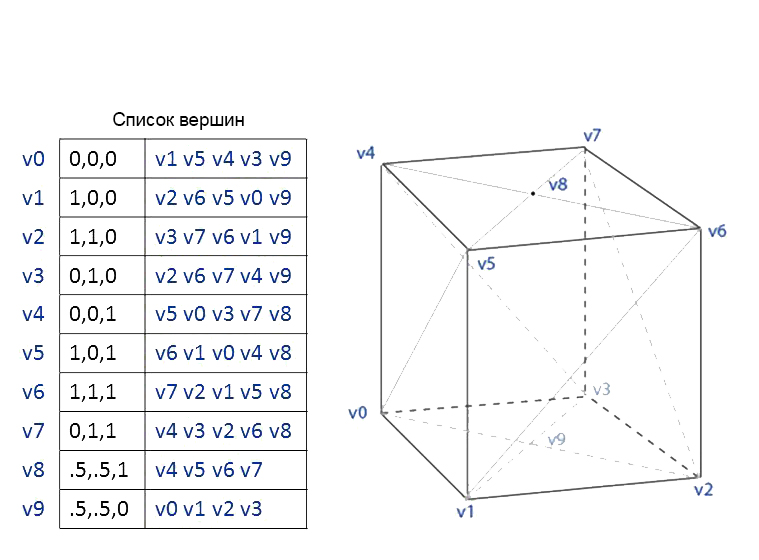
\includegraphics[width=0.9\textwidth]{vertex}
	\caption{"Представление точка-точка"}
	\label{fig:vertex-vertex}
\end{figure}


\subsubsection{Представление точка-грань}
Представление "точка-грань" описывает поверхность с помощью списка точек и граней. При этом для каждой грани хранятся образующие точки, а для каждой точки соседние грани. За счёт избыточности в хранении, получается упростить операции над гранями поверхности, однако для получения рёбер потребуется пройти по всем точкам грани. Представление продемонстрировано на рисунке \ref{fig:vertex-face}.

\begin{figure}[h]
	\centering
	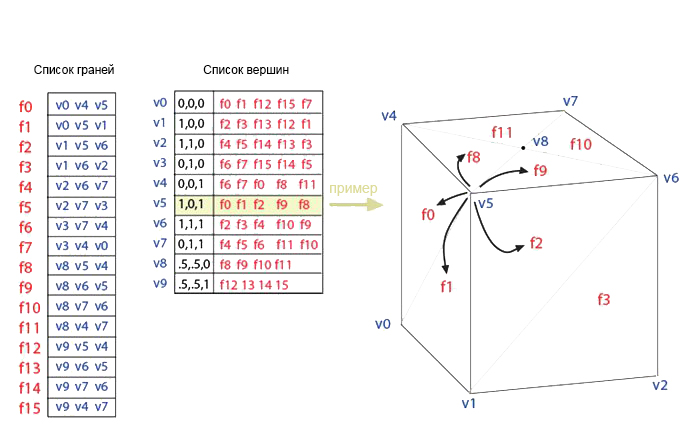
\includegraphics[width=0.9\textwidth]{faces}
	\caption{"Представление точка-грань"}
	\label{fig:vertex-face}
\end{figure}

\subsubsection{"Крылатое" представление}
При крылатом представлении центральным объектом являются рёбра, при этом для каждого ребра хранятся две точки, образующие его, две грани, которые образует он и 4 ребра, которые с ним соединены c ним, по 2 с каждой точкой. Так как количество соседних рёбер может быть больше 2-х, то для каждого ребра хранятся ближайшие ребра по часовой и против часовой стрелок.
Представление требует больше памяти для хранения, но упрощает некоторые операции над моделями.
Представление продемонстрировано на рисунке \ref{fig:winged}.

\begin{figure}[h]
	\centering
	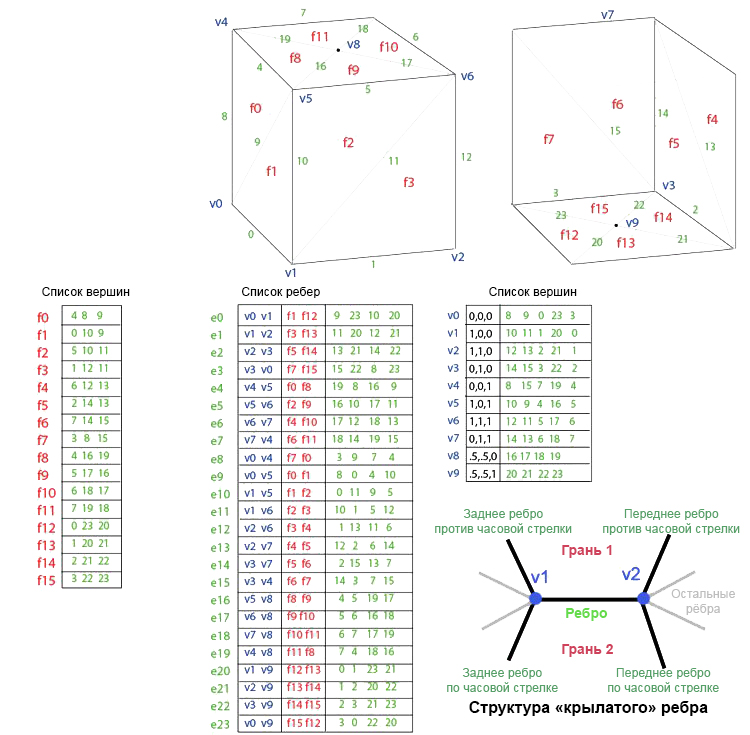
\includegraphics[width=0.9\textwidth]{winged}
	\caption{"Крылатое представление"}
	\label{fig:winged}
\end{figure}


Для данной работы имеет смысл использовать представление моделей с помощью полигональной сетки, чтобы сделать тела отличающимися не только по цвету, но и по форме, что упростит визуальные различия тел при визуализации.

В качестве представления сетки оптимально использовать список граней, так как при динамической отрисовке объектов потребуется информация о гранях, которая не хранится явно в представлении "точка-точка". "крылатое"  представление является избыточным в данном случае, так как операции по преобразованию моделей не планируются в этой работе.

\section{Алгоритмы удаления невидимых поверхностей}

Алгоритм удаления невидимых поверхностей является
центральным этапом при визуализации сцены. При этом также она является наиболее вычислительно сложной в компьютерной графике \cite{rodgers}. На данном этапе определяются объекты или, в некоторых алгоритмах, части объектов, которые буду отрисованы на экране.

Классифицировать алгоритмы можно по системе координат, в которой они работают:
\begin{itemize}
	\item\textbf{В пространстве объектов} - имеют дело с физической системой координат, в которой заданы объекты. Точность ограничена точностью вычислений.
	\item\textbf{В пространстве экрана} - имеют дела с системой координат, связанной с экраном, то есть сначала объекты проецируются на экран, а затем уже выполняется удаление невидимых объектов. Точность ограничена разрешением экрана.
\end{itemize}
Рассмотрим некоторые алгоритмы подробнее.

\subsection{Алгоритмы в объектном пространстве}
\subsubsection{Алгоритм Робертса}
Алгоритм Робертса - первое известное решение задачи удаления невидимых поверхностей. Для работы алгоритма требуются выпуклые тела. Алгоритм состоит из 4-х этапов.

\textbf{Первый этап} - подготовка матрицы тела. Матрица тела - матрица, хранящая информацию об уравнениях, задающих плоскости всех граней. Имеет размерность $4*n$, где n - число граней тела.

\begin{equation}
	\label{eq:body_matrix}
	V = \begin{pmatrix}
		a_1\ a_2\ \dots\ a_n \\
		b_1\ b_2\ \dots\ b_n \\
		c_1\ c_2\ \dots\ c_n \\
		d_1\ d_2\ \dots\ d_n 
	\end{pmatrix},
\end{equation}
где $ a_ix + b_iy + c_iz + d_i = 0 $ - уравнение i-ой грани. Матрица должна быть сформирована так, чтобы при умножению на неё точку внутри тела получался вектор положительных чисел. Для проверки можно использовать пробную точку, при этом с учётом того, что тела выпуклые, можно взять геометрический центр фигуры. Если какое-то значение вектора отрицательно для пробной точки, то соответствующий столбец матрицы нужно умножить на -1.

\textbf{Второй этап} - удаление нелицевых граней. На данном этапе удаляются грани, которые экранируются самими объектами. Для этого берётся вектор взгляда $E = (0, 0,-1, 0)$ и умножается на матрицу тела. Отрицательные столбцы полученного вектора будут соответствовать невидимым граням, так как вектор взгляда разнонаправлен с внутренней нормалью.

\textbf{Третий этап} - удаление рёбер, экранируемых другими телами. Для этого для каждого оставшегося ребра нужно пустить луч из точки взгляда к точке ребра. Если луч проходит через другие грани, значит эта точка отрезка экранируется. 

\textbf{Четвёртый этап} - создание рёбер соединения граней. Для этого запоминаются все точки протыкания в предыдущем пункте и попарно соединяются отрезками. Далее эти отрезки также проверяются на экранирование, как и 3-ем пункте.

Алгоритм обеспечивает высокую точность вычислений, но сложный вычислительно и налагает условие выпуклости на тела.


\subsubsection{Алгоритм трассировки лучей}

Алгоритм трассировки лучей основан на идее, что наблюдатель видит объекты, от которых отразился луч света от некоторого источника света. Поэтому для построения сцены требуется проследить лучи по законам оптики из всех источников света до наблюдателя.

Основным недостатком алгоритма является большое число лучей для обработки. При этом большинство этих лучей уйдёт на неотражающие и непрозрачные объекты или на бесконечность, то есть не внесут ничего в сцену.

\subsubsection{Алгоритм обратной трассировки лучей}
Если в алгоритме трассировке лучей прослеживается путь от источника света через объекты до наблюдателя, то в алгоритме обратной трассировке лучей прослеживается лучи из наблюдателя, проходящие через пиксель экрана, до объекта. При этом уже до полученной точки объекта рассматривается луч освещения. Для расчёта отражений объекта луч можно продолжить по законам отражения после первого пересечения, при этом учтя интенсивность последующих объектов с меньшей интенсивностью.

Алгоритм потенциально эффективнее чем прямой метод, но тем не менее все равно требует много вычислений, так как расчёты с лучами достаточно сложные. \cite{rodgers}


\subsection{Алгоритмы в пространстве экрана}
\subsubsection{Алгоритм Варнока}

Алгоритм Варнока основан на идее, что для обработки областей с малой плотностью информации мозг человека тратит малое количество времени, а с большой плотностью — больше.

Данный алгоритм работает в пространстве изображения, то есть с проекциями объектов на экран и с самим экраном. Идея алгоритма в том, чтобы разбивать экран на окна и подокна до тех пор, пока его содержимое не будет элементарным для визуализации, или пока не будет достигнут предел разрешения. На рисунке \ref{fig:varnok} представлен пример разбиения экрана алгоритмом Варнока.

\begin{figure}[h]
	\centering
	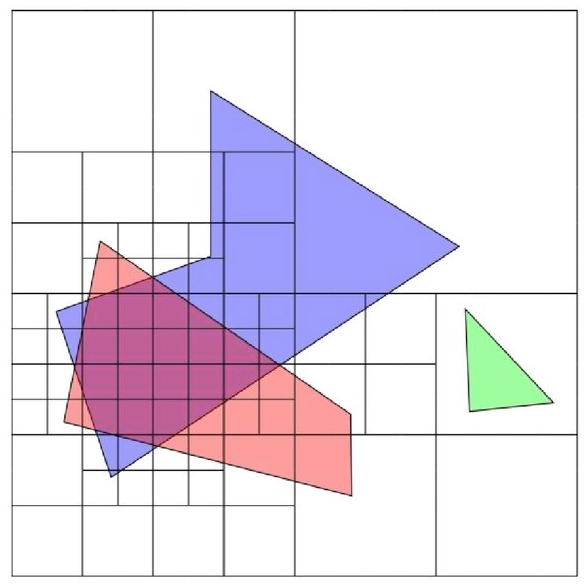
\includegraphics[width=0.9\textwidth]{varnok}
	\caption{"Пример работы алгоритма Варнока"}
	\label{fig:varnok}
\end{figure}

\subsubsection{Алгоритм использующий z-буфер}
Алгоритм z-буфера — один из простейших и широко используемых алгоритмов отрисовки удаления невидимых поверхностей.

Основой алгоритма является два буфера, оба имеют размеры экрана в пикселях:

\begin{itemize}
	\item \textbf{Буфер кадра} — используется для хранения значения интенсивности(цвета) каждого пикселя, который будет отрисован на экране. По сути хранит в себе то, как экран будет выглядеть в следующем кадре.
	\item \textbf{Буфер глубины(z-буфер)} — Используется для хранения глубины каждого пикселя, описанного в буфере кадра. Нужен для определения видимых граней.
\end{itemize}

По умолчанию буфер кадра заполнен интенсивностью фона, а буфер глубины значением бесконечности.
По ходу, алгоритм проецирует грани на экран и пытается занести проекцию в буфер кадра. Если для соответствующих x и y точки проекцию глубина больше, чем глубина анализируемой точки, то текущее значение записывается в буфер кадра. Иначе значение в буфере кадра не меняется, так как до этого была точка, которая ближе текущей, а значит перекрывает её.

Главное преимущество алгоритма — простота. Алгоритм легко решает задачу удаления невидимых поверхностей. Трудоёмкость алгоритма увеличивается линейно, при увеличении числа объектов на сцене. Также алгоритму не нужна предварительная сортировка по глубине, что повышает его эффективность, по сравнению с другими алгоритмами. Но при этом алгоритм требует большего объёма памяти, для хранения буферов \cite{rodgers}.

\subsection{Выбор алгоритма удаления невидимых поверхностей}


Таким образом для данной работы является оптимальным использование алгоритма использующего z-буфер. Алгоритм достаточно прост и популярен, что делает его относительно простым в реализации, при этом он эффективнее других алгоритмов, ценой затратами памяти.


\section{Модели освещения}
Модели освещения в компьютерной графике делятся на 2 больших класса: глобальные и локальные.

Глобальные модели освещения учитывают не только свет от прямых источников, но и отражённый или преломлённый от других объектов. Например от прозрачных объектов, которые пропускают часть цвета, преломляя его, или от зеркальной поверхности, которая почти полностью его отражают. Расчёт такой модели требует больших вычислительных затрат и реализуется с помощью алгоритмов трассировок лучей. Так как в данной работе сцена динамическая и не используется трассировка лучей, то для неё лучше подходят локальные модели освещения.

Локальные модели освещения учитывают только прямой свет от источника до рассматриваемого объекта. Такие модели можно использовать без трассировки лучей и они рассчитываются быстрее.

\subsection{Модель Ламберта}
Свет от источника может быть поглощён, отражён или пропущен телом. Пропускание света требует трассировки лучей, поэтому не рассматривается в локальных моделях.

Отражённый свет зависит от характеристик и положения источника, относительно тела. Отражённый свет бывает диффузным или зеркальным. Диффузное отражение вызывается колебаниями заряженных частиц поверхности тела, которые вызываются поглощением исходного света от источника. При этом свет испускается во все стороны равномерно. Рассчитать интенсивность отражаемого света можно по закону Ламберта:
\begin{equation}
	\label{eq:lambert1}
	I = I_{l}k_dcos(\phi),\ 0\leq\phi\leq\frac{\pi}{2},
\end{equation}
где $I$ - интенсивность отражённого света, $I_s$ - интенсивность источника света, $k_d$ - коэффициент диффузного отражения тела, $\phi$ - угол между нормалью к поверхности в точке падения и направлением света.

В реальности на объекты падает свет от других объектов, но его точный просчёт сложен, поэтому в локальных моделях он заменяется на рассеянный свет:
\begin{equation}
	\label{eq:lambert2}
	I = I_ak_a + I_{l}k_dcos(\phi),\ 0\leq\phi\leq\frac{\pi}{2},
\end{equation}
где $I_a$ - интенсивность рассеянного света, $k_a$ - коэффициент диффузного отражения рассеянного света. 

\subsection{Модель Фонга}
В отличие от диффузного отражения, зеркальное является направленным, при этом вектор отражения лежит в плоскости, а угол между нормалью и вектором отражения равен углу между нормалью и углом падения. Если вектор наблюдателя не совпадает с вектором отражения, то и зеркального отражения не видно. Модель Фонга для зеркального отражения имеет вид:

\begin{equation}
	\label{eq:fong-reflection}
	I_s = I_{l}k_scos^n(\alpha),
\end{equation}
где $k_s$ - коэффициент зеркального отражения, $\alpha$ - угол между лучом отражения и лучом наблюдателя, $n$ - степень пространственного отражения.

Объединив с диффузным отражением по формуле \ref{eq:lambert2}, получим модель освещения Фонга:

\begin{equation}
	\label{eq:fong-model}
	I = I_ak_a + I_{l}(k_dcos(\phi) + k_scos^n(\alpha))
\end{equation}

\section{Методы закраски}
Методы закраски описывают то, как будут закрашены грани тел, в зависимости падающего на них света.

\subsection{Простая закраска}
При простой закраске нормаль считается одинаковой для всех точек грани. Соответственно цвет в конкретной точке зависит только от расстояния до источника освещения.
При такой закраске все грани будут чётко видны, что в случае полигональной аппроксимации тел, например тел вращения, может дать нереалистичную картину. Тем не менее, по сравнению с остальными закрасками метод прост в реализации и быстрее остальных в вычислениях.

\subsection{Закраска по Гуро}
В отличие от простой закраски, закраска по Гуро закрашивает грани разной интенсивностью. Для этого рассчитывается интенсивность в вершинах грани, а затем используется билинейная интерполяция для расчёта интенсивности в конкретной точке.
Сначала интенсивность линейно интерполируется в точках пересечения сканирующей строки с рёбрами грани. Затем интерполируется между полученными точками пересечения в требуемой точке. Полученная картина сглажена по всей поверхности и это скрывает аппроксимацию тел гранями.

Недостатком метода является то, что он не учитывает изменение вектора нормали по всей поверхности, поэтому при учёте зеркальной составляющей блики будут выглядеть размыто и нереалистично.

На рисунке \ref{fig:guro_inter} представлен пример расчёта закраски по Гуро. Сначала рассчитывается интенсивность в вершинах грани, затем интерполируется в точках a и b. Затем вдоль сканирующей  интенсивность интерполируется для искомой точки p.

\begin{figure}[h]
	\centering
	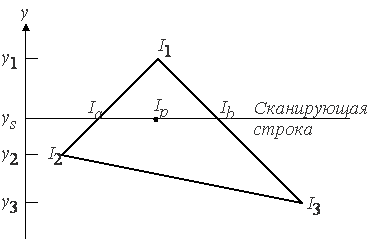
\includegraphics[width=0.9\textwidth]{guro_inter}
	\caption{"Расчёт интенсивности методом Гуро"}
	\label{fig:guro_inter}
\end{figure}

\subsection{Закраска по Фонгу}
Закраска по Фонгу учитывает изменение нормаль поверхности и позволяет лучше учитывать зеркальное отражение. Она также как и закраска по Гуро использует билинейную интерполяцию, однако интерполирует не интенсивность, а нормаль к плоскости. Это увеличивает количество вычислений, но позволяет улучшить зеркальное отражение, то есть блики.

На рисунке \ref{fig:shading} представлено сравнение описанных выше методов закраски, как видно закраски по Гуро и Фонгу действительно сглаживают фигуру, но у закраски по Гуро блик сосредоточен вокруг вершины и нереалистично расходится, в то время как у Фонга он выглядит более правильной формы.

\begin{figure}[h]
	\centering
	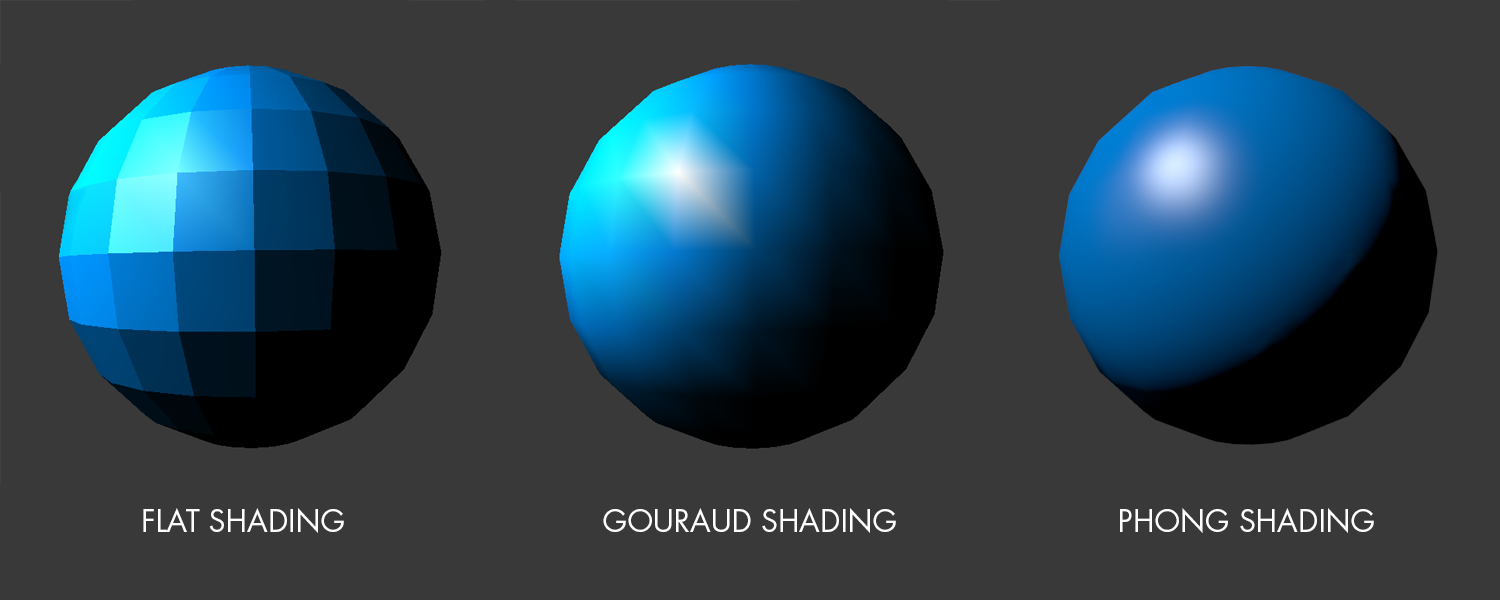
\includegraphics[width=0.9\textwidth]{Shading_models}
	\caption{"Сравнение методов закраски на примере аппроксимации шара"}
	\label{fig:shading}
\end{figure}

\section{Вывод по моделям освещения и метода закраски}

С точки зрения качества визуализации комбинация модели освещения Фонга и закраски по Фонгу, так как такая комбинация позволяет получить более реалистичную и качественную картину. Но в данной работе я отдам предпочтение простой закраске с освещением Фонга, так как:
\begin{itemize}
	\item Простая закраска быстрее других видов;
	\item В работе не планируется использовать тела вращения, а только многогранники.
\end{itemize}




\section{Алгоритм учёта теней}

Существуют разные способы учёта теней в сценах. Самый очевидный из них, протрассировать лучи от каждого источника света до точки, для которой рассчитывается тень. Если на пути встречается хотя бы один объект, то относительно этого источника точка находится в тени. Однако такой метод требует высоких вычислительных затрат. Такой метод хорошо подходит при алгоритмах трассировки лучей, так как в данных методах все равно приходится просчитывать лучи.

Часто для быстрого учёта теней используют другие методы, позволяющие упростить вычисления ценой точностью сцены. Для этого тени делят на проекционные и собственные. Собственные тени образуются телами на себя, проекционные - образованные другими телами. Для расчёта собственных теней можно использовать первые два этапа алгоритма Робертса из положения источника света. Нелицевые грани относительно источника света будут затенёнными.

Для учёта как проекционных, так собственных теней можно использовать метод теневых карт \cite{gabriella}. Данный метод работает похоже с методом z-буфера. Для каждого точечного источника света пространство делится на 6 частей, в виде прямоугольного параллелепипед вокруг точки. В каждом из четырёх направлений строится буфер глубины без буфера интенсивности. Затем при построении буфера из наблюдателя, если точка видна, она линейно преобразуется в пространство источника света. Если в пространстве света она ближе, чем значение в буфере глубины, то точка освещена, иначе в тени.

В данной работе будет использоваться метод теневых карт, так как он является расширением метода буфера глубины, которые будет использоваться в работе.

\section*{Вывод}

В результате аналитической части были описаны теоретические сведения о способах представления объектов программно и методы преобразования этих объектов для отображения на экране. Также были выбраны методы, которые будут использоваться в данной работе.

\clearpage
